\chapter{The GPT Architecture}

The previous chapters built the pieces: token data, tensors, embeddings, layer normalization, causal self-attention, MLPs, and residual connections. This chapter assembles those pieces into one complete GPT model.

A GPT model is not mysterious when viewed as a contract:

\begin{quote}
Given token IDs with shape \shape{[B,T]}, produce vocabulary logits with shape \shape{[B,T,V]}, and optionally compute next-token loss against targets with shape \shape{[B,T]}.
\end{quote}

The architecture is a disciplined stack of repeated blocks. The power comes not from a single complicated operation, but from repeating simple operations at scale.

\section{Chapter Goals}

By the end of this chapter, you should be able to:

\begin{itemize}
  \item draw the full GPT forward pass from token IDs to logits;
  \item explain every major configuration field in TinyGPT;
  \item map model configuration to tensor shapes and source-code modules;
  \item explain why logits have shape \shape{[B,T,V]};
  \item estimate the parameter count of a GPT model;
  \item describe initialization, dropout, weight tying, and checkpoint contents;
  \item read a complete TinyGPT module implementation block by block;
  \item state the architecture contract shared by PyTorch, Candle, and C/CUDA backends.
\end{itemize}

\section{The Whole Model At A Glance}

TinyGPT follows this path:

\begin{lstlisting}
token ids
-> token embedding + position embedding
-> Transformer block 1
-> Transformer block 2
-> ...
-> final LayerNorm
-> language-model head
-> logits over vocabulary
-> optional cross-entropy loss
\end{lstlisting}

\begin{center}
\resizebox{\textwidth}{!}{
\begin{tikzpicture}[
  box/.style={draw, rounded corners=2pt, minimum height=0.66cm, text width=2.0cm, align=center},
  arrow/.style={-{Latex[length=2mm]}, thick},
  note/.style={font=\small, align=center}
]
\node[box, fill=blue!5] (ids) at (0,0) {token IDs\\\shape{[B,T]}};
\node[box, fill=blue!5] (emb) at (2.5,0) {token + position\\\shape{[B,T,C]}};
\node[box, fill=red!8] (b1) at (5.0,0) {block 1\\\shape{[B,T,C]}};
\node[box, fill=red!8] (b2) at (7.5,0) {block 2\\\shape{[B,T,C]}};
\node[box, fill=gray!12] (dots) at (9.7,0) {\(\cdots\)};
\node[box, fill=red!8] (bn) at (11.9,0) {block \(N\)\\\shape{[B,T,C]}};
\node[box, fill=yellow!18] (ln) at (14.4,0) {final LN\\\shape{[B,T,C]}};
\node[box, fill=green!10] (head) at (16.9,0) {LM head\\\shape{[B,T,V]}};
\draw[arrow] (ids) -- (emb);
\draw[arrow] (emb) -- (b1);
\draw[arrow] (b1) -- (b2);
\draw[arrow] (b2) -- (dots);
\draw[arrow] (dots) -- (bn);
\draw[arrow] (bn) -- (ln);
\draw[arrow] (ln) -- (head);
\node[note] at (8.4,-1.0) {The shape stays \shape{[B,T,C]} inside the Transformer stack. Only the final head changes \(C\) into \(V\).};
\end{tikzpicture}}
\end{center}

The main data transformation is:

\[
\mathbb{Z}^{B\times T}
\rightarrow
\mathbb{R}^{B\times T\times C}
\rightarrow
\mathbb{R}^{B\times T\times V}.
\]

\section{The TinyGPT Configuration}

A model configuration is not paperwork. It defines the size and legal behavior of every tensor in the model.

\begin{longtable}{p{0.23\textwidth}p{0.18\textwidth}p{0.45\textwidth}}
\toprule
\term{Field} & \term{Tiny value} & \term{Meaning} \\
\midrule
\texttt{vocab\_size} & 9 & number of tokenizer tokens \(V\) \\
\texttt{block\_size} & 4 or 5 & maximum context length \(T_{\max}\) \\
\texttt{n\_layer} & 2 & number of Transformer blocks \(N\) \\
\texttt{n\_head} & 2 & number of attention heads \(H\) \\
\texttt{n\_embd} & 6 & hidden width \(C\) \\
\texttt{dropout} & 0.0 or 0.1 & random activation dropping during training \\
\texttt{bias} & true/false & whether linear layers include bias vectors \\
\bottomrule
\end{longtable}

\begin{center}
\begin{tikzpicture}[
  box/.style={draw, rounded corners=2pt, minimum height=0.62cm, text width=2.2cm, align=center},
  arrow/.style={-{Latex[length=2mm]}, thick},
  note/.style={font=\small, align=center}
]
\node[box, fill=blue!5] (cfg) at (0,0) {config};
\node[box, fill=red!8] (data) at (3,1.2) {data contract\\\(V,T\)};
\node[box, fill=red!8] (model) at (3,0) {model size\\\(N,H,C\)};
\node[box, fill=red!8] (train) at (3,-1.2) {training behavior\\dropout, bias};
\node[box, fill=green!10] (ckpt) at (6.2,0) {checkpoint\\interpretation};
\draw[arrow] (cfg) -- (data);
\draw[arrow] (cfg) -- (model);
\draw[arrow] (cfg) -- (train);
\draw[arrow] (data) -- (ckpt);
\draw[arrow] (model) -- (ckpt);
\draw[arrow] (train) -- (ckpt);
\node[note] at (3,-2.05) {Weights are only meaningful together with the config that shaped them.};
\end{tikzpicture}
\end{center}

If a checkpoint contains a tensor of shape \shape{[9,6]} for token embeddings, the model must know that \(V=9\) and \(C=6\). If the tokenizer changes, the rows may refer to different tokens.

\section{Configuration As Source Code}

A minimal configuration object:

\begin{lstlisting}[language=Python]
from dataclasses import dataclass

@dataclass
class GPTConfig:
    vocab_size: int = 9
    block_size: int = 5
    n_layer: int = 2
    n_head: int = 2
    n_embd: int = 6
    dropout: float = 0.0
    bias: bool = True
\end{lstlisting}

The configuration also imposes constraints. For attention:

\[
C \mod H = 0.
\]

The head dimension is:

\[
d=\frac{C}{H}.
\]

For TinyGPT:

\[
C=6,\quad H=2,\quad d=3.
\]

\begin{center}
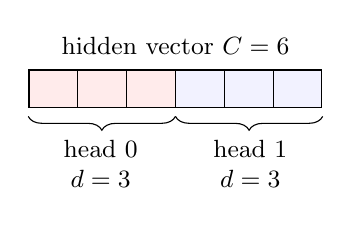
\begin{tikzpicture}[
  cell/.style={draw, minimum width=0.62cm, minimum height=0.48cm, align=center},
  note/.style={font=\small, align=center}
]
\node[note] at (1.55,0.55) {hidden vector \(C=6\)};
\foreach \i in {0,1,2,3,4,5} {
  \ifnum\i<3
    \node[cell, fill=red!8] at (\i*0.62,0) {};
  \else
    \node[cell, fill=blue!5] at (\i*0.62,0) {};
  \fi
}
\draw[decorate, decoration={brace, mirror, amplitude=5pt}] (-0.32,-0.35) -- (1.55,-0.35);
\draw[decorate, decoration={brace, mirror, amplitude=5pt}] (1.55,-0.35) -- (3.42,-0.35);
\node[note] at (0.6,-0.95) {head 0\\\(d=3\)};
\node[note] at (2.5,-0.95) {head 1\\\(d=3\)};
\end{tikzpicture}
\end{center}

\section{Module Tree: What Owns What}

A GPT model is an \texttt{nn.Module}. It owns child modules, and child modules own parameters.

\begin{center}
\resizebox{\textwidth}{!}{
\begin{tikzpicture}[
  box/.style={draw, rounded corners=2pt, minimum height=0.62cm, text width=2.4cm, align=center},
  arrow/.style={-{Latex[length=2mm]}, thick}
]
\node[box, fill=blue!5] (gpt) at (0,0) {\texttt{TinyGPT}};
\node[box, fill=red!8] (tok) at (3,1.8) {\texttt{tok\_emb}\\\shape{[V,C]}};
\node[box, fill=red!8] (pos) at (3,0.9) {\texttt{pos\_emb}\\\shape{[Tmax,C]}};
\node[box, fill=yellow!18] (blocks) at (3,0) {\texttt{blocks}\\list of \(N\)};
\node[box, fill=red!8] (ln) at (3,-0.9) {\texttt{ln\_f}\\final norm};
\node[box, fill=green!10] (head) at (3,-1.8) {\texttt{lm\_head}\\\shape{[V,C]}};
\node[box, fill=gray!12] (attn) at (6,0.6) {attention\\QKV + proj};
\node[box, fill=gray!12] (mlp) at (6,-0.3) {MLP\\up + GELU + down};
\node[box, fill=gray!12] (lns) at (6,-1.2) {LayerNorms};
\draw[arrow] (gpt) -- (tok);
\draw[arrow] (gpt) -- (pos);
\draw[arrow] (gpt) -- (blocks);
\draw[arrow] (gpt) -- (ln);
\draw[arrow] (gpt) -- (head);
\draw[arrow] (blocks) -- (attn);
\draw[arrow] (blocks) -- (mlp);
\draw[arrow] (blocks) -- (lns);
\end{tikzpicture}}
\end{center}

This ownership tree matters for:

\begin{itemize}
  \item collecting parameters with \texttt{model.parameters()};
  \item saving checkpoints with \texttt{state\_dict()};
  \item moving the whole model to a device with \texttt{model.to(device)};
  \item switching dropout behavior with \texttt{model.train()} and \texttt{model.eval()}.
\end{itemize}

\section{Forward Pass Math}

Let input token IDs be:

\[
x\in\mathbb{Z}^{B\times T}.
\]

The model first computes token and position embeddings:

\[
X_0 = E_{\text{tok}}[x] + E_{\text{pos}}[0:T-1].
\]

Then it applies \(N\) Transformer blocks:

\[
X_{\ell}=\operatorname{Block}_{\ell}(X_{\ell-1}),\qquad \ell=1,\ldots,N.
\]

After the last block:

\[
H=\operatorname{LN}_{f}(X_N).
\]

The language-model head produces logits:

\[
Z=HW_{\text{out}}^\top + b_{\text{out}}.
\]

The shape is:

\[
Z\in\mathbb{R}^{B\times T\times V}.
\]

\begin{center}
\resizebox{\textwidth}{!}{
\begin{tikzpicture}[
  box/.style={draw, rounded corners=2pt, minimum height=0.66cm, text width=2.05cm, align=center},
  arrow/.style={-{Latex[length=2mm]}, thick},
  note/.style={font=\small, align=center}
]
\node[box, fill=blue!5] (x) at (0,0) {\(x\)\\\(\mathbb{Z}^{B\times T}\)};
\node[box, fill=blue!5] (x0) at (2.8,0) {\(X_0\)\\\(\mathbb{R}^{B\times T\times C}\)};
\node[box, fill=red!8] (x1) at (5.6,0) {\(X_1\)};
\node[box, fill=red!8] (x2) at (8.4,0) {\(\cdots X_N\)};
\node[box, fill=yellow!18] (h) at (11.2,0) {\(H\)\\final LN};
\node[box, fill=green!10] (z) at (14.0,0) {\(Z\)\\\(\mathbb{R}^{B\times T\times V}\)};
\draw[arrow] (x) -- node[above, font=\small] {embedding} (x0);
\draw[arrow] (x0) -- node[above, font=\small] {block 1} (x1);
\draw[arrow] (x1) -- node[above, font=\small] {blocks} (x2);
\draw[arrow] (x2) -- node[above, font=\small] {normalize} (h);
\draw[arrow] (h) -- node[above, font=\small] {head} (z);
\node[note] at (7,-1.0) {The model preserves batch and time axes. It changes feature interpretation layer by layer.};
\end{tikzpicture}}
\end{center}

\section{Forward Pass Source Code}

A compact TinyGPT forward method:

\begin{lstlisting}[language=Python]
def forward(self, idx, targets=None):
    # idx: [B, T]
    B, T = idx.shape
    assert T <= self.config.block_size

    pos = torch.arange(0, T, device=idx.device)    # [T]
    tok = self.tok_emb(idx)                        # [B, T, C]
    pos = self.pos_emb(pos)                        # [T, C]
    x = self.drop(tok + pos)                       # [B, T, C]

    for block in self.blocks:
        x = block(x)                               # [B, T, C]

    x = self.ln_f(x)                               # [B, T, C]
    logits = self.lm_head(x)                       # [B, T, V]

    loss = None
    if targets is not None:
        loss = F.cross_entropy(
            logits.view(B * T, -1),
            targets.view(B * T)
        )
    return logits, loss
\end{lstlisting}

The model has two modes:

\begin{itemize}
  \item \term{training/evaluation mode}: call with \texttt{idx} and \texttt{targets}; return logits and loss;
  \item \term{generation mode}: call with only \texttt{idx}; return logits and no loss.
\end{itemize}

\section{Why Logits Have Three Axes}

The logits tensor has shape:

\[
\shape{[B,T,V]}.
\]

Each axis has a specific meaning:

\begin{longtable}{p{0.14\textwidth}p{0.22\textwidth}p{0.48\textwidth}}
\toprule
\term{Axis} & \term{Name} & \term{Meaning} \\
\midrule
\(B\) & batch & which sequence example \\
\(T\) & time & which token position in the context \\
\(V\) & vocabulary & one score for every possible next token \\
\bottomrule
\end{longtable}

\begin{center}
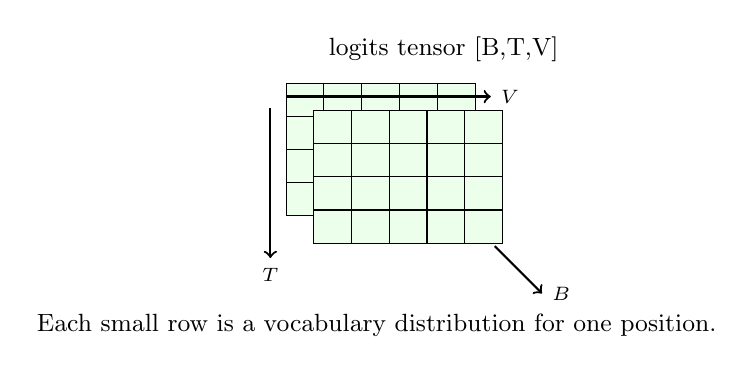
\begin{tikzpicture}[
  cell/.style={draw, minimum width=0.54cm, minimum height=0.40cm, align=center},
  note/.style={font=\small, align=center}
]
\node[note] at (2.0,0.85) {logits tensor \shape{[B,T,V]}};
\foreach \b/\shift in {0/0,1/0.35} {
  \foreach \t in {0,1,2,3} {
    \foreach \v in {0,1,2,3,4} {
      \draw[fill=green!8] (\v*0.48+\shift,-\t*0.42-\shift) rectangle +(0.48,0.42);
    }
  }
}
\draw[->, thick] (-0.2,0.1) -- (-0.2,-1.8) node[below] {\scriptsize \(T\)};
\draw[->, thick] (0,0.25) -- (2.6,0.25) node[right] {\scriptsize \(V\)};
\draw[->, thick] (2.65,-1.65) -- (3.25,-2.25) node[right] {\scriptsize \(B\)};
\node[note] at (1.15,-2.65) {Each small row is a vocabulary distribution for one position.};
\end{tikzpicture}
\end{center}

For TinyGPT with \(B=2\), \(T=4\), and \(V=9\):

\[
\text{logits shape}=\shape{[2,4,9]}.
\]

This means there are \(2\times4=8\) next-token predictions in the batch, each with 9 token scores.

\section{From Logits To Loss}

Targets have shape:

\[
y\in\mathbb{Z}^{B\times T}.
\]

The loss compares every position's logits with the correct next-token ID. PyTorch cross entropy expects:

\[
\text{logits as } \shape{[B T,V]},
\qquad
\text{targets as } \shape{[B T]}.
\]

\begin{center}
\resizebox{0.96\textwidth}{!}{
\begin{tikzpicture}[
  box/.style={draw, rounded corners=2pt, minimum height=0.66cm, text width=2.25cm, align=center},
  arrow/.style={-{Latex[length=2mm]}, thick},
  note/.style={font=\small, align=center}
]
\node[box, fill=green!10] (logits) at (0,0.7) {logits\\\shape{[B,T,V]}};
\node[box, fill=blue!5] (targets) at (0,-0.7) {targets\\\shape{[B,T]}};
\node[box, fill=yellow!18] (flat1) at (3.2,0.7) {flatten\\\shape{[B*T,V]}};
\node[box, fill=yellow!18] (flat2) at (3.2,-0.7) {flatten\\\shape{[B*T]}};
\node[box, fill=red!8] (ce) at (6.3,0) {cross entropy};
\node[box, fill=gray!12] (loss) at (9.0,0) {loss\\scalar};
\draw[arrow] (logits) -- (flat1);
\draw[arrow] (targets) -- (flat2);
\draw[arrow] (flat1) -- (ce);
\draw[arrow] (flat2) -- (ce);
\draw[arrow] (ce) -- (loss);
\node[note] at (4.6,-1.55) {The training batch becomes many independent next-token classification examples.};
\end{tikzpicture}}
\end{center}

For one position:

\[
L=-\log p_{\text{correct}}.
\]

For the whole batch:

\[
L_{\text{batch}}=
\frac{1}{BT}
\sum_{b=1}^{B}\sum_{t=1}^{T}
-\log p_{b,t,y_{b,t}}.
\]

\section{Parameter Groups Inside GPT}

The parameters are not evenly distributed. Most parameters live in large matrices.

\begin{longtable}{p{0.22\textwidth}p{0.24\textwidth}p{0.38\textwidth}}
\toprule
\term{Component} & \term{Approx count} & \term{Purpose} \\
\midrule
Token embeddings & \(VC\) & map token IDs to vectors \\
Position embeddings & \(T_{\max}C\) & encode positions \\
Attention QKV & \(3C^2\) per block & create queries, keys, values \\
Attention output & \(C^2\) per block & mix heads back to hidden width \\
MLP up projection & \(4C^2\) per block & expand features \\
MLP down projection & \(4C^2\) per block & compress features back to \(C\) \\
LayerNorm & small, \(O(C)\) & stabilize activations \\
Output head & \(VC\), if untied & map hidden states to vocabulary logits \\
\bottomrule
\end{longtable}

\begin{center}
\resizebox{0.95\textwidth}{!}{
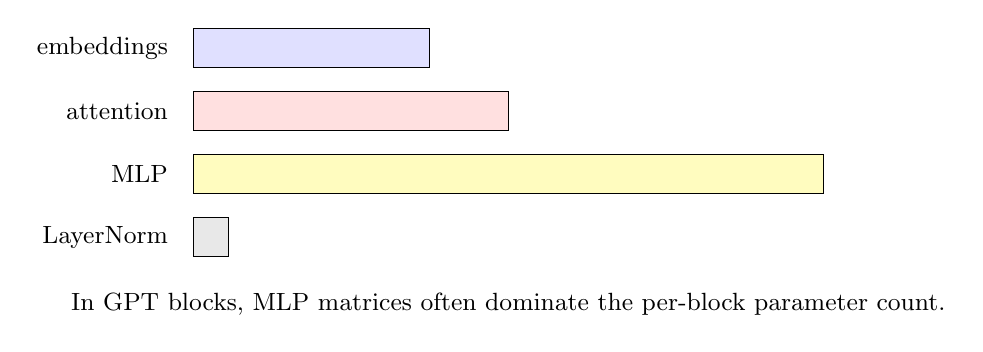
\begin{tikzpicture}[
  bar/.style={draw, minimum height=0.5cm, anchor=west},
  note/.style={font=\small, align=center}
]
\node[note, anchor=east] at (0,0) {embeddings};
\draw[bar, fill=blue!12] (0.2,-0.25) rectangle +(3.0,0.5);
\node[note, anchor=east] at (0,-0.8) {attention};
\draw[bar, fill=red!12] (0.2,-1.05) rectangle +(4.0,0.5);
\node[note, anchor=east] at (0,-1.6) {MLP};
\draw[bar, fill=yellow!25] (0.2,-1.85) rectangle +(8.0,0.5);
\node[note, anchor=east] at (0,-2.4) {LayerNorm};
\draw[bar, fill=gray!18] (0.2,-2.65) rectangle +(0.45,0.5);
\node[note] at (4.2,-3.25) {In GPT blocks, MLP matrices often dominate the per-block parameter count.};
\end{tikzpicture}}
\end{center}

\section{Parameter Count Approximation}

Ignoring small bias and LayerNorm terms, each Transformer block has:

\[
3C^2 + C^2 + 4C^2 + 4C^2 = 12C^2
\]

parameters.

With \(N\) layers:

\[
\text{block params}\approx 12NC^2.
\]

Add embeddings:

\[
\text{embedding params}=VC+T_{\max}C.
\]

If the output head is not tied to the token embedding table, add another \(VC\). If tied, do not add it again.

\subsection{TinyGPT Count}

For:

\[
V=9,\quad T_{\max}=5,\quad C=6,\quad N=2,
\]

embedding parameters:

\[
VC+T_{\max}C=9\cdot6+5\cdot6=84.
\]

block parameters:

\[
12NC^2=12\cdot2\cdot6^2=864.
\]

Approximate total with tied output head:

\[
84+864=948.
\]

The exact count differs because of biases and LayerNorm parameters, but the estimate teaches scale.

\subsection{A Small Practical Count}

For:

\[
V=8192,\quad T_{\max}=256,\quad C=256,\quad N=4,
\]

\[
VC=8192\cdot256=2{,}097{,}152,
\]

\[
T_{\max}C=256\cdot256=65{,}536,
\]

\[
12NC^2=12\cdot4\cdot256^2=3{,}145{,}728.
\]

Approximate total:

\[
5{,}308{,}416.
\]

This is small for modern LLMs, but large enough for students to see real training behavior.

\section{Initialization}

Training begins with random weights. Random does not mean careless. If weights are too large, activations and gradients can explode. If weights are too small, signals may shrink and learning can be slow.

A common GPT-style initialization is:

\[
W\sim\mathcal{N}(0,0.02^2).
\]

In code:

\begin{lstlisting}[language=Python]
def _init_weights(self, module):
    if isinstance(module, nn.Linear):
        torch.nn.init.normal_(module.weight, mean=0.0, std=0.02)
        if module.bias is not None:
            torch.nn.init.zeros_(module.bias)
    elif isinstance(module, nn.Embedding):
        torch.nn.init.normal_(module.weight, mean=0.0, std=0.02)
\end{lstlisting}

\begin{center}
\begin{tikzpicture}[
  box/.style={draw, rounded corners=2pt, minimum height=0.65cm, text width=2.4cm, align=center},
  arrow/.style={-{Latex[length=2mm]}, thick},
  note/.style={font=\small, align=center}
]
\node[box, fill=blue!5] (rand) at (0,0) {small random\\weights};
\node[box, fill=yellow!18] (forward) at (3.1,0) {stable-ish\\activations};
\node[box, fill=red!8] (loss) at (6.2,0) {loss creates\\gradients};
\node[box, fill=green!10] (learn) at (9.3,0) {optimizer shapes\\useful weights};
\draw[arrow] (rand) -- (forward);
\draw[arrow] (forward) -- (loss);
\draw[arrow] (loss) -- (learn);
\node[note] at (4.65,-0.95) {Initialization starts the search; training discovers useful structure.};
\end{tikzpicture}
\end{center}

For deep GPTs, some implementations scale residual projection initialization. The intuition is that many residual branches are added together, so their variance should not grow too quickly with depth.

\section{Dropout}

Dropout randomly zeros some activations during training:

\[
\tilde{x}_i =
\begin{cases}
0, & \text{with probability }p,\\
\dfrac{x_i}{1-p}, & \text{with probability }1-p.
\end{cases}
\]

The scaling keeps the expected activation roughly unchanged.

\begin{center}
\begin{tikzpicture}[
  cell/.style={draw, minimum width=0.62cm, minimum height=0.48cm, align=center},
  arrow/.style={-{Latex[length=2mm]}, thick},
  note/.style={font=\small, align=center}
]
\foreach \i/\v in {0/0.2,1/-0.1,2/0.5,3/0.3,4/-0.4,5/0.1} {
  \node[cell, fill=blue!5] at (\i*0.62,0) {\scriptsize \v};
}
\node[note] at (1.55,0.65) {before dropout};
\node[draw, rounded corners=2pt, fill=yellow!18, minimum width=1.6cm, minimum height=0.65cm, align=center] (drop) at (4.8,0) {dropout};
\foreach \i/\v/\col in {0/0.25/green!10,1/0.00/gray!18,2/0.63/green!10,3/0.00/gray!18,4/-0.50/green!10,5/0.13/green!10} {
  \node[cell, fill=\col] at (6.2+\i*0.62,0) {\scriptsize \v};
}
\node[note] at (7.75,0.65) {during training};
\draw[arrow] (3.8,0) -- (drop);
\draw[arrow] (drop) -- (5.75,0);
\end{tikzpicture}
\end{center}

In tiny educational runs, set dropout to \(0\) when checking whether the model can overfit a tiny batch. Dropout intentionally makes memorization harder, which can hide basic bugs.

During validation or sampling:

\begin{lstlisting}[language=Python]
model.eval()
\end{lstlisting}

This disables dropout and uses deterministic behavior.

\section{Weight Tying In The Full Model}

Chapter 5 introduced weight tying. In the full architecture, tied weights mean the input token embedding and output head share the same parameter tensor.

\begin{lstlisting}[language=Python]
self.tok_emb = nn.Embedding(config.vocab_size, config.n_embd)
self.lm_head = nn.Linear(config.n_embd, config.vocab_size, bias=False)
self.lm_head.weight = self.tok_emb.weight
\end{lstlisting}

\begin{center}
\resizebox{0.86\textwidth}{!}{
\begin{tikzpicture}[
  box/.style={draw, rounded corners=2pt, minimum height=0.66cm, text width=2.35cm, align=center},
  arrow/.style={-{Latex[length=2mm]}, thick},
  note/.style={font=\small, align=center}
]
\node[box, fill=blue!5] (ids) at (0,0) {input IDs};
\node[box, fill=red!8] (emb) at (3,0) {shared token table\\\shape{[V,C]}};
\node[box, fill=yellow!18] (blocks) at (6,0) {GPT blocks};
\node[box, fill=red!8] (head) at (9,0) {same table\\used as head};
\node[box, fill=green!10] (logits) at (12,0) {logits};
\draw[arrow] (ids) -- (emb);
\draw[arrow] (emb) -- (blocks);
\draw[arrow] (blocks) -- (head);
\draw[arrow] (head) -- (logits);
\draw[<->, thick, dashed] (emb.south) .. controls (5,-1.1) and (7,-1.1) .. (head.south);
\node[note] at (6,-1.45) {One parameter matrix serves reading and scoring.};
\end{tikzpicture}}
\end{center}

This reduces parameters and often improves training behavior, but it must be recorded in config because it changes checkpoint interpretation.

\section{Complete TinyGPT Module}

Putting the pieces together:

\begin{lstlisting}[language=Python]
class TinyGPT(nn.Module):
    def __init__(self, config):
        super().__init__()
        self.config = config

        self.tok_emb = nn.Embedding(config.vocab_size, config.n_embd)
        self.pos_emb = nn.Embedding(config.block_size, config.n_embd)
        self.drop = nn.Dropout(config.dropout)
        self.blocks = nn.ModuleList([Block(config) for _ in range(config.n_layer)])
        self.ln_f = nn.LayerNorm(config.n_embd)
        self.lm_head = nn.Linear(config.n_embd, config.vocab_size, bias=False)

        self.lm_head.weight = self.tok_emb.weight
        self.apply(self._init_weights)

    def forward(self, idx, targets=None):
        B, T = idx.shape
        assert T <= self.config.block_size

        pos = torch.arange(0, T, device=idx.device)
        x = self.tok_emb(idx) + self.pos_emb(pos)
        x = self.drop(x)

        for block in self.blocks:
            x = block(x)

        x = self.ln_f(x)
        logits = self.lm_head(x)

        loss = None
        if targets is not None:
            loss = F.cross_entropy(logits.view(B*T, -1), targets.view(B*T))

        return logits, loss
\end{lstlisting}

\section{Checkpoint Contents}

A checkpoint should contain enough information to resume or interpret training:

\begin{itemize}
  \item model weights;
  \item optimizer state, if resuming training;
  \item model configuration;
  \item tokenizer metadata;
  \item training step and token count;
  \item random seeds or reproducibility notes;
  \item validation loss history, if available.
\end{itemize}

\begin{center}
\begin{tikzpicture}[
  box/.style={draw, rounded corners=2pt, minimum height=0.62cm, text width=2.5cm, align=center},
  arrow/.style={-{Latex[length=2mm]}, thick}
]
\node[box, fill=blue!5] (weights) at (0,1.2) {model\\weights};
\node[box, fill=yellow!18] (opt) at (0,0) {optimizer\\state};
\node[box, fill=red!8] (cfg) at (0,-1.2) {config +\\tokenizer};
\node[box, fill=green!10] (ckpt) at (4,0) {checkpoint\\file};
\node[box, fill=gray!12] (resume) at (8,0.7) {resume\\training};
\node[box, fill=gray!12] (sample) at (8,-0.7) {load for\\sampling};
\draw[arrow] (weights) -- (ckpt);
\draw[arrow] (opt) -- (ckpt);
\draw[arrow] (cfg) -- (ckpt);
\draw[arrow] (ckpt) -- (resume);
\draw[arrow] (ckpt) -- (sample);
\end{tikzpicture}
\end{center}

Saving only weights is sometimes enough for inference, but it is not enough for serious training practice.

\section{Architecture Contract Across Backends}

The same model family can have multiple implementations:

\begin{lstlisting}
torch_reference   -> easiest to read and debug
candle_rust       -> Rust-native implementation path
llmc_cuda         -> low-level systems/performance path
\end{lstlisting}

They should agree on the architecture contract:

\begin{longtable}{p{0.24\textwidth}p{0.26\textwidth}p{0.34\textwidth}}
\toprule
\term{Contract item} & \term{Shape or type} & \term{Meaning} \\
\midrule
input IDs & \shape{[B,T]} integer & tokenized context windows \\
targets & \shape{[B,T]} integer & shifted next-token IDs \\
logits & \shape{[B,T,V]} float & scores for vocabulary tokens \\
loss & scalar float & mean cross-entropy \\
checkpoint config & structured data & model and tokenizer meaning \\
\bottomrule
\end{longtable}

\begin{center}
\resizebox{0.95\textwidth}{!}{
\begin{tikzpicture}[
  box/.style={draw, rounded corners=2pt, minimum height=0.66cm, text width=2.35cm, align=center},
  arrow/.style={-{Latex[length=2mm]}, thick}
]
\node[box, fill=blue!5] (contract) at (0,0) {architecture\\contract};
\node[box, fill=red!8] (torch) at (3.3,1.0) {PyTorch\\reference};
\node[box, fill=green!10] (candle) at (3.3,0) {Candle\\Rust};
\node[box, fill=gray!12] (cuda) at (3.3,-1.0) {C/CUDA\\systems};
\node[box, fill=yellow!18] (tests) at (6.7,0) {shared tests\\shape, loss,\\sampling};
\draw[arrow] (contract) -- (torch);
\draw[arrow] (contract) -- (candle);
\draw[arrow] (contract) -- (cuda);
\draw[arrow] (torch) -- (tests);
\draw[arrow] (candle) -- (tests);
\draw[arrow] (cuda) -- (tests);
\end{tikzpicture}}
\end{center}

This is how a repo becomes more than a pile of code. It becomes a training pack with a stable model specification.

\section{Engineering Practice}

Recommended repository organization:

\begin{lstlisting}
mapletrain/
  torch_reference/
    model.py
    attention.py
    train.py
  candle_backend/
    src/
  cuda_backend/
    csrc/
configs/
  tiny.yaml
  small.yaml
scripts/
  train_torch.py
  sample_torch.py
  inspect_tokens.py
checkpoints/
  torch/
  candle/
\end{lstlisting}

Architecture tests should verify:

\begin{itemize}
  \item logits shape is \shape{[B,T,V]};
  \item loss is scalar when targets are provided;
  \item generation mode works without targets;
  \item tied weights are actually shared when configured;
  \item block size errors are caught early;
  \item checkpoint config matches the model object;
  \item parameter count is close to expected.
\end{itemize}

\section{Hands-On Lab: Assemble TinyGPT}

Build a minimal TinyGPT configuration:

\begin{lstlisting}[language=Python]
config = GPTConfig(
    vocab_size=9,
    block_size=5,
    n_layer=2,
    n_head=2,
    n_embd=6,
    dropout=0.0,
)
\end{lstlisting}

Then create a toy batch:

\begin{lstlisting}[language=Python]
idx = torch.tensor([[2, 3, 4, 5, 6],
                    [3, 4, 5, 6, 7]], dtype=torch.long)
targets = torch.tensor([[3, 4, 5, 6, 7],
                        [4, 5, 6, 7, 8]], dtype=torch.long)
\end{lstlisting}

Run:

\begin{lstlisting}[language=Python]
model = TinyGPT(config)
logits, loss = model(idx, targets)

print("logits:", logits.shape)
print("loss:", loss.item())
print("parameters:", sum(p.numel() for p in model.parameters()))
print("tied:", model.lm_head.weight is model.tok_emb.weight)
\end{lstlisting}

Expected:

\begin{lstlisting}
logits: [2, 5, 9]
loss: a scalar number
tied: True
\end{lstlisting}

\checkpoint

\begin{enumerate}
  \item What is the full GPT data path from token IDs to logits?
  \item Why is configuration part of the model, not just a training detail?
  \item If \(C=768\) and \(H=12\), what is the head dimension \(d\)?
  \item Why does the hidden tensor stay \shape{[B,T,C]} through the Transformer stack?
  \item What does each axis of \shape{[B,T,V]} mean?
  \item Why does the loss flatten logits to \shape{[B*T,V]}?
  \item Why is \(12NC^2\) a useful parameter-count estimate?
  \item Why should a checkpoint store tokenizer metadata?
  \item Why should dropout be disabled during sampling?
  \item What should remain consistent across PyTorch, Candle, and C/CUDA backends?
\end{enumerate}

\subsection*{Solutions}

\begin{enumerate}
  \item Token IDs go through token and position embeddings, repeated Transformer blocks, final LayerNorm, and the language-model head to produce vocabulary logits.
  \item Configuration defines tensor shapes, number of layers, attention heads, vocabulary size, and interpretation of weights. Without it, the weights cannot be safely understood.
  \item \(d=C/H=768/12=64\).
  \item Each block is designed to return the same hidden shape it receives. This lets blocks be stacked repeatedly.
  \item \(B\) selects the batch example, \(T\) selects the token position, and \(V\) selects the vocabulary score.
  \item Cross entropy treats each row as one classification example. The \(B\times T\) token positions become \(B T\) next-token predictions.
  \item Each block contains roughly \(4C^2\) attention parameters and \(8C^2\) MLP parameters, so \(N\) blocks give about \(12NC^2\).
  \item Embedding rows correspond to tokenizer IDs. If tokenizer metadata is missing or wrong, the same row may refer to the wrong token.
  \item Dropout is random during training. Sampling should be deterministic except for the intentional sampling procedure itself.
  \item They should share input shapes, target shapes, logits shape, loss definition, tokenizer/config contract, and checkpoint meaning.
\end{enumerate}
